% !TEX root = ../../main.tex

\begin{figure*}[t]
    \centering 
    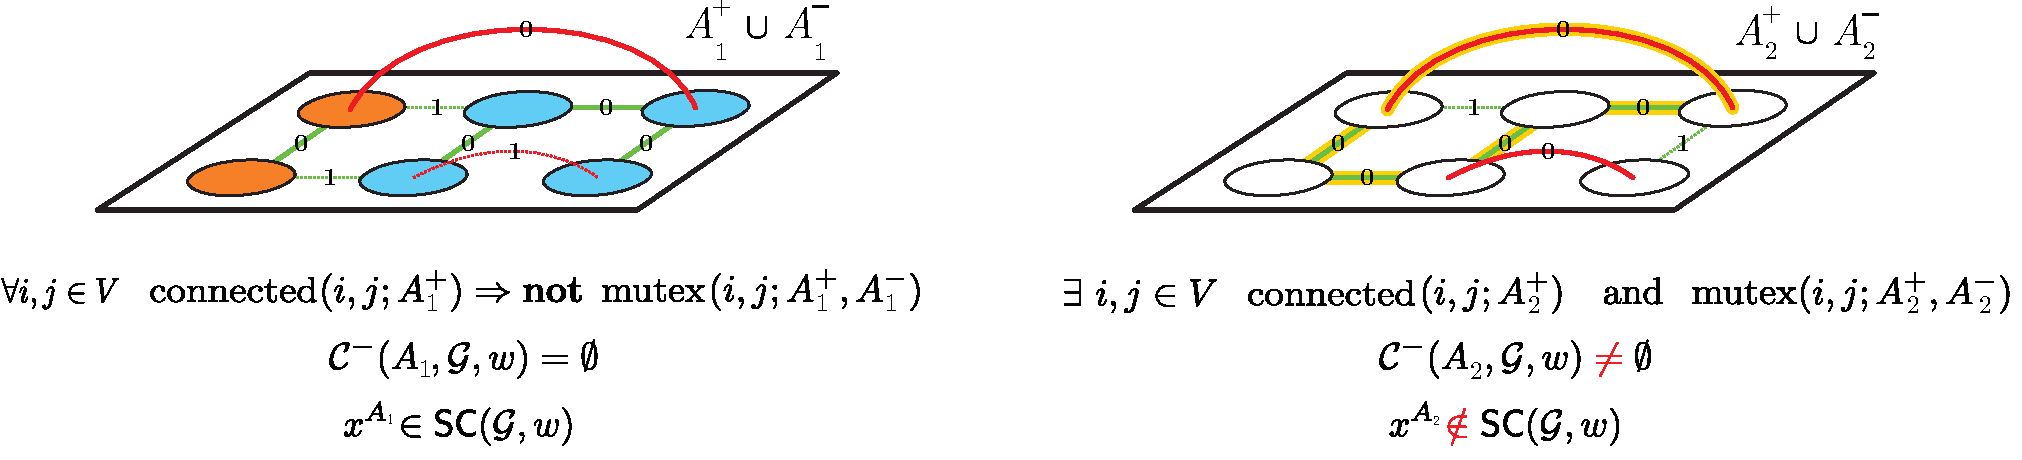
\includegraphics[width=\linewidth]{figures/MWS/images/consistent-sets-combined.pdf}
    % \begin{subfigure}[t]{0.45\textwidth}
    %     \centering
    %     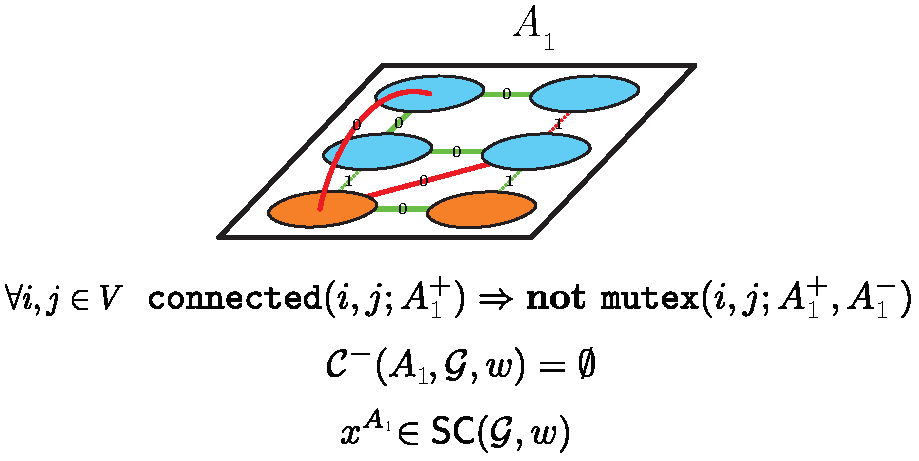
\includegraphics[width=\linewidth]{images/consistent-sets.pdf}
    %     % \caption{Consistent active sets}
    %     % $\mathcal{C}^-(A, \mathcal{G},w)=\emptyset \quad x^A\in \mathsf{SC}(\mathcal{G}, w)\quad \operator{connected}(i, j; A^+) \Rightarrow \textbf{not } \operator{mutex}(i, j; A^+,A^-)$.
    % \end{subfigure}%
    % \hfill 
    % \begin{subfigure}[t]{0.45\textwidth}
    %     \centering
    %     \includegraphics[width=\linewidth]{images/inconsistent-sets.pdf}
    %     % \caption{$\mathcal{C}^-(A, \mathcal{G},w)\neq \emptyset \quad x^A\notin \mathsf{SC}(\mathcal{G}, w)\quad \operator{connected}(i, j; A^+) \nRightarrow \textbf{not } \operator{mutex}(i, j; A^+,A^-)$}
    % \end{subfigure} \hfill 
    \caption{\textbf{Consistent and inconsistent active sets} -- Two different active edge sets $A_1\subseteq E$ (on the left) and $A_2\subseteq E$ (on the right) on identical toy graphs with six nodes, attractive~(green) and repulsive~(red) edges. The value of the edge indicator $x^A\in \{0,1\}^{|E|}$ defined in Eq.~\ref{def:active_edge_indicator} is shown for every edge. Members of the active sets are shown as solid lines.  \textbf{On the left}, the active set $A_1$ is \emph{consistent}, i.e. does not include any conflicted cycle $\mathcal{C}^-(\mathcal{G},w)$ (see Def. \ref{def:conflicted_cycles}): Therefore, it is associated with a clustering (represented by arbitrary node colors). \textbf{On the right}, the active set $A_2$ is not consistent and includes at least one conflicted cycle (highlighted in yellow), thus it cannot be associated with a node clustering.}
\label{fig:conflicted_cycles}
\end{figure*}


\section{Theoretical characterization}\label{sec:MWS_objective}

\noindent \textbf{Towards the Multicut framework.}
In section \ref{3_3_MWS}, we have introduced the Mutex Watershed (MWS) algorithm as a generalization of seeded watersheds and the Kruskal algorithm in particular. 
However, since we are considering graphs with negative edge weights, the MWS is conceptually closer to the multicut problem and related heuristics such as GAEC and GF \cite{levinkov2017comparative}.
Fortunately, due to the structure of the MWS it can be analyzed using dynamic programming. This section summarizes our second contribution, i.e. the proof that the Mutex Watershed Algorithm globally optimizes a precise objective related to the multicut.

\subsection{Review of the Multicut problem and its objective}
In the following, we will review the multicut problem not in its standard formulation but in the \textit{Cycle Covering Formulation} introduced in \cite{lange2018partial}, which is similar to the MWS formulation as it also considers the set of \textit{attractive} and \textit{repulsive} edges separately. 
Previously, in Sec.~\ref{sec:notation}, we defined a clustering by introducing the concept of an active set of edges \mbox{$A=A^+\cup A^-\subseteq E$} and the \operator{connected/}\operator{mutex} predicates. In particular, an active set describes a valid clustering if it does not include \textbf{both} a path of only attractive edges \textbf{and} a path with exactly one repulsive edge connecting any two nodes $i,j\in V$:
\begin{equation}
\operator{connected}(i, j; A^+) \quad \Longrightarrow \quad \textbf{not } \operator{mutex}(i, j; A^+,A^-).
\end{equation}
In other words, an active set is \emph{consistent} and describes a clustering if it does not contain any cycle with exactly one repulsive edge (known as conflicted cycles). 

\begin{definition} \label{def:conflicted_cycles}
\textbf{Conflicted cycles} --
We call a cycle of $\mathcal{G}$ conflicted w.r.t. $(\mathcal{G},w)$ if it contains precisely one repulsive edge $e \in E^-$, s.t. $w_e < 0$. We denote by $\mathcal{C}^-(\mathcal{G},w) \subseteq \mathcal{C}(\mathcal{G},w)$ the set of all conflicted cycles. Furthermore, given a set of edges $A \subseteq E$, we denote by $\mathcal{C}^-(A, \mathcal{G},w) \subseteq \mathcal{C}^-(\mathcal{G},w)$ the set of conflicted cycles involving only edges in $A$.
\end{definition}

\noindent 
From now on, in order to describe different clustering solutions in the framework of (integer) linear programs, we associate each active set $A$ with the following edge indicator $x^A$
\begin{equation}
         x^A := \mathbbm{1}\{e \notin A)\} \in \{0,1\}^{|E|}. \label{def:active_edge_indicator}
\end{equation}
In this way, the cycle-free property $\mathcal{C}^-(A, \mathcal{G},w)=\emptyset$ of an active set can be reformulated in terms of linear inequalities:
\begin{equation}
\forall C \in \mathcal{C}^-(\mathcal{G},w): \sum_{e\in E_C} x^A_e \geq 1 \quad \Longleftrightarrow \quad \mathcal{C}^-(A, \mathcal{G},w) = \emptyset. \label{eq:cycles_and_linear_ineq}
\end{equation}
In words, the active set cannot contain conflicted cycles; or vice versa, every conflicted cycle must contain at least one edge that is not part of the active set.
Following \cite{lange2018partial}, via this property we describe the space of all possible clustering solutions by defining the convex hull $\mathsf{SC}(\mathcal{G}, w)$ of all edge indicators corresponding to valid clusterings of $(\mathcal{G}, w)$:
\begin{definition}\label{def:set_covering_hull}
Let $\mathsf{SC}(\mathcal{G}, w)$ denote the convex hull of all edge indicators \mbox{$x \in \{0,1\}^{|E|}$} satisfying the following system of inequalities:
\begin{equation} 
\forall C \in \mathcal{C}^-(\mathcal{G},w): \quad \sum_{e\in E_C} x_e \geq 1. \label{eq:def_set_covering_hull}
\end{equation} 
That is, $\mathsf{SC}(\mathcal{G}, w)$ contains all edge labelings for which every conflicted cycle is broken at least once. We call $\mathsf{SC}(\mathcal{G}, w)$ the set covering polyhedron with respect to conflicted cycles, similarly to \cite{lange2018partial}.
\end{definition}


\noindent Fig.~\ref{fig:conflicted_cycles} summarizes these definitions and provides an example of consistent and inconsistent active sets with their associated clusterings and edge indicators.  

As shown in \cite{lange2018partial}, the \emph{multicut optimization problem} can be formulated with constraints over conflicted cycles in terms of the following integer linear program (ILP), which is NP-hard:
\begin{gather}
\min_{x \in \mathsf{SC}(\mathcal{G},w)} \sum_{e\in E} |w_e| x_e.
\label{eq:MC_set_covering_problem}
\end{gather}
The solution of the multicut problem is given by the clustering associated to the connected components of the active set $\hat{A}^+=\{e\in E^+|\hat{x}_e=0\}$, where \mbox{$\hat{x} \in \{0,1\}^{|E|}$} is the solution of (\ref{eq:MC_set_covering_problem}).

\subsection{Mutex Watershed Objective}\label{sec:MWS_objective_sub}

We now define the Mutex Watershed objective that is minimized by the Mutex Watershed Algorithm~(proof in \autoref{sec:optimality_MWS}) and show how it is closely related to the multicut problem defined in Eq. (\ref{eq:MC_set_covering_problem}). 
Lange et al.\ \cite{lange2018partial} introduce the concept of dominant edges in a graph. For example, an attractive edge $f \in E^+$ is called dominant if 
there exists a cut $B$ with $f \in E_B$ such that 
$|w_{f}| \geq \sum_{e \in E_{B} \backslash\{f\}}\left|w_{e}\right|$.
\REVIEW{These highlight an aspect of the multicut problem that can be used to search for optimal solutions more efficiently.}
Not all weighted graphs contain dominant edges; but if, assuming no ties, we raise all graph weights to a large enough power a similar property emerges.
\begin{definition}\label{def:pineq}
\textbf{Dominant power:}
Let $\mathcal{G} = (V, E, w)$ be an edge-weighted graph, with unique weights $w: E \rightarrow \mathbb{R}$. We call $p \in \mathbb{N}^+$ a dominant power if:
\begin{equation}
    |w_e|^p > \sum_{t \in E,\; w_t < w_e} |w_t|^p \qquad \forall e \in E, \label{eq:pcondition}
\end{equation}
\end{definition}
 \noindent In contrast to dominant edges \cite{lange2018partial}, we do not consider edges on a cut but rather all edges with smaller absolute weight. Note that there exists a dominant power for any finite set of edges, since for any $e \in E$ we can divide (\ref{eq:pcondition}) by $|w_e|^p$ and observe that the normalized weights $|w_t|^p/|w_e|^p$ (and any finite sum of these weights) converges to 0 when $p$ tends to infinity. 

 By considering the multicut problem in Eq. (\ref{eq:MC_set_covering_problem}) and raising the weights $|w_e|$ to a dominant power $p$, we fundamentally change the problem structure:
 \begin{definition}\label{def:MWS_objective}
\textbf{Mutex Watershed Objective:}
Let $\mathcal{G} = (V, E, w)$ be an edge-weighted graph, with unique weights $w:E \rightarrow \mathbb{R}$ and $p \in \mathbb{N}^+$ a dominant power. Then the Mutex Watershed Objective is defined as the integer linear program
\begin{equation}
  \min_{x \in \mathsf{SC}(\mathcal{G}, w)} \quad \sum_{e \in E}  |w_e|^p \, x_e  \label{eq:MWS_objective_SC}
\end{equation}
where $\mathsf{SC}(\mathcal{G}, w)$ is the convex hull defined in Def.~\ref{def:set_covering_hull}.
\end{definition}

In the following section, we will prove that this modified version of the multicut objective, which we call Mutex Watershed Objective, is indeed optimized by the Mutex Watershed Algorithm:

\begin{restatable}{theorem}{Objective}\label{theo:optimal_v1}
Let $\mathcal{G} = (V, E, w)$ be an edge-weighted graph, with unique weights $w:E \rightarrow \mathbb{R}$ and $p \in \mathbb{N}^+$ a dominant power. Then the edge indicator given by the Mutex Watershed Algorithm \ref{algo_code_efficient} $$x^{\mathbf{MWS}} := \mathbbm{1}\Big\{e \notin \mathbf{MWS}\Big(\mathcal{G}, w, \operator{connect\_all=True}\Big)\Big\}$$ minimizes the Mutex Watershed Objective in Eq.~(\ref{eq:MWS_objective_SC}).
\end{restatable} 
\noindent 

\subsection{Proof of optimality via dynamic programming} \label{sec:optimality_MWS}

\begin{algorithm}[t]
  \caption{Conflicted-Cycles Mutex Watershed}
  \begin{algorithmic}[1]
      \Procedure{ConflictedCyclesMWS}{$\mathcal{G}(V,E),w:E\rightarrow \mathbb{R}$}
      \State $A \leftarrow \emptyset$\;
      \For{$(i,j) = e \in E $ {\rm in descending order of } $|w_e|$}     
          \If{\rm $\mathcal{C}^-(A\cup \{e\},\mathcal{G},w) = \emptyset$}
              \State $A \leftarrow A \cup e$
          \EndIf
        \EndFor
        \State
        \Return $A$
      \EndProcedure
  \end{algorithmic}
    \label{MWS_conflicted_cycles}
\algcomment{Equivalent formulation of the Mutex Watershed Algorithm \ref{algo_code_efficient}, \REVIEW{with input parameter $\operator{connect\_all=True}$}. The set of conflicted cycles $\mathcal{C}^-(A,\mathcal{G},w)$ is defined in Def. \ref{def:conflicted_cycles}. The output clustering is defined by the connected components of the final attractive active set $A^+=A\cap E^+$.}

\end{algorithm}


% \begin{algorithm}[b]
%  \hrulefill \\
%  \textbf{Conflicted-Cycles Mutex Watershed:}\\
% \SetKwProg{CCMWS}{CCMWS}{$\big(\mathcal{G}(V,E),w:E\rightarrow \mathbb{R}\big)$:}{}
% \CCMWS{}{
%  $A \leftarrow \emptyset$\;
%  \For{$(i,j) = e \in E $ {\rm in descending order of } $|w_e|$} 
%  {
%     \If{\rm $\mathcal{C}^-(A\cup \{e\},\mathcal{G},w) = \emptyset$}{
%           $A \leftarrow A \cup e$\;
    
%     }
%  }
%  \Return $A$\;
%  }
%   \vspace{3pt}
% \hrulefill
%  \vspace{3pt}
%  \caption{Equivalent formulation of the Mutex Watershed Algorithm \ref{algo_code_efficient}, \REVIEW{with input parameter $\operator{connect\_all=True}$}. The set of conflicted cycles $\mathcal{C}^-(A,\mathcal{G},w)$ is defined in Def. \ref{def:conflicted_cycles}. The output clustering is defined by the connected components of the final attractive active set $A^+=A\cap E^+$.}
%  \label{MWS_conflicted_cycles}
% % }
% \end{algorithm}

In this section we prove Theorem \ref{theo:optimal_v1}, i.e.\ that the Mutex Watershed Objective defined in \ref{def:MWS_objective} is solved to optimality by the Mutex Watershed Algorithm \ref{MWS_conflicted_cycles}. Particularly, in the following Sec.~\ref{sec:cycle_consistency} we show that the edge indicator associated to the solution of the MWS algorithm lies in $\mathsf{SC}(\mathcal{G},w)$, whereas in Sec.~\ref{sec:optimilaty_proof} we prove that it solves Eq.~\ref{eq:MWS_objective_SC} to optimality.


% In this section we reformulate the Mutex Watershed Algorithm \ref{algo_code_efficient} \REVIEW{ in the framework of graph cuts and express the ``connected'' and ``mutex'' predicates introduced in Section~\ref{sec:notation} using ``conflicted''\cite{lange2018partial} (also known as ``erroneous''\cite{demaine2006correlation}) cycles:}

% \BIG{We show that $ x^{\mathit{MWS}} \in \mathsf{SC}(\mathcal{G}, w) $ by}
% \BIG{1) defining $\mathsf{SC}$ using $\mathcal{C}^-$}
% \BIG{rewriting \autoref{MWS_conflicted_cycles}}

% \operator{\,\,is\,consistent}

% It then follows that  we consider the integer edge indicator $x \in \{0,1\}^{|E|}$ such that each edge in the set is labeled with zero, i.e. $x =\mathds{1}\{e\notin A\}$, then we can rewrite the condition $\mathcal{C}^-(A, \mathcal{G},w)=\emptyset$ in terms of the following system of inequalities  (\ref{eq:def_set_covering_hull})
% In particular, 

\subsubsection{Cycle consistency}\label{sec:cycle_consistency}
The Mutex Watershed algorithm introduced in Sec.~\ref{3_methods} iteratively builds an active set $A = A^+ \cup A^-$ such that nodes engaged in a mutual exclusion constraint (encoded by edges in $A^-$) are never part of the same cluster. In other words, this means that the active set built by the Mutex Watershed at every iteration does never include a \emph{conflicted cycle} and is always \emph{consistent}. 
In particular, for any attractive edge $(i,j) = e^+ \in E^+$ and any consistent set $A$ that fulfills $\mathcal{C}^-(A,\mathcal{G},w) = \emptyset$:
\begin{align*}
\mathbf{not }\operator{ mutex}(i, j, A^+, A^-)\quad \Leftrightarrow &\quad \mathcal{C}^-(A\cup \{e^+\},\mathcal{G},w) = \emptyset 
\intertext{Similarly, for any repulsive edge $(s,t) = e^- \in E^-$:}
\mathbf{not} \operator{ connected}(s, t, A^+) \quad \Leftrightarrow &\quad \mathcal{C}^-(A\cup \{e^-\},\mathcal{G},w) = \emptyset
\end{align*}

\noindent Therefore, we can rewrite Algorithm~\ref{algo_code_efficient}  in the form of Algorithm~\ref{MWS_conflicted_cycles}. 
This new formulation makes it clear that 
\begin{equation}
    \mathcal{C}^-\Big(\mathbf{MWS}\big(\mathcal{G}, w, \operator{connect\_all=True}\big)\Big) = \emptyset.
\end{equation}
Thus, thanks to Eq.~\ref{eq:cycles_and_linear_ineq} and definition \ref{def:set_covering_hull}, it follows that the MWS edge indicator $x^{\mathbf{MWS}}$ defined in \ref{theo:optimal_v1} lies in  $\mathsf{SC}(\mathcal{G},w)$:
\begin{equation}
    x^{\mathbf{MWS}} \in \mathsf{SC}(\mathcal{G},w).
\end{equation}


\subsubsection{Optimality}\label{sec:optimilaty_proof}
We first note that the Mutex Watershed Objective \ref{def:MWS_objective} and Theorem~\ref{theo:optimal_v1} can easily be reformulated in terms of active sets to minimize 
\begin{equation}
  \argmin_{A \subseteq E} \quad - \sum_{e \in A}  |w_e|^p  \qquad \operator{s.t.} \quad \mathcal{C}^-(A,\mathcal{G},w)=\emptyset.  \label{eq:full_problem_active_set}
\end{equation}
% \TODO{I think this is }
% \begin{restatable}{theorem}{Objective_v2}\label{theo:optimal_v2}
% Let $\mathcal{G} = (V, E, w)$ be an edge-weighted graph, with unique weights $w:E \rightarrow \mathbb{R}$ and $p \in \mathbb{N}^+$ a dominant power. Then the final active set $A^*$ of the Mutex Watershed Algorithm \ref{MWS_conflicted_cycles} is given by the following minimization problem:
% \begin{equation}
%   \argmin_{A \subseteq E} \quad - \sum_{e \in A}  |w_e|^p  \qquad \operator{s.t.} \quad \mathcal{C}^-(A,\mathcal{G},w)=\emptyset.  \label{eq:full_problem_active_set}
% \end{equation}
% This theorem is equivalent to Theorem~\ref{theo:optimal_v1} thanks to Property~\ref{set_of_all_consistent_sets}. 
% \end{restatable} 




\noindent We now generalize the Mutex Watershed (see Algorithm~\ref{algo_subproblems}) and the objective such that an initial consistent set of active edges $\Ainit \subseteq E$ is supplied:

\begin{definition} \label{def:general_MWS_obj}
\textbf{Energy optimization subproblem.}
% Given a graph $G = (V, E^+ \cup E^-)$, let us consider the set ${\sigma := \langle e_1,e_2,\ldots,e_M \rangle}$ of edges in $E$ sorted in descending order by their weight $W^+ \cup W^-$. The integer index $j_{e} \in \mathbb{N}$ denotes the sorting index of the edge $e$, so that $\sigma_{j_{e}}=e$. 
Let \mbox{$\mathcal{G} = (V, E, w)$} be an edge-weighted graph. Define the optimal solution of the subproblem as
\begin{gather} \label{eq:general_MWS_obj}
  \subproblem(\mathcal{G},\Ainit) := \underset{A \subseteq (E \setminus \Ainit)}{\text{argmin}} \; T(A) \qquad \operator{with} \quad T(A) := - \sum_{e \in A} |w_e|^p, \\
  \operator{s.t.} \quad \mathcal{C}^{-}(A \cup \Ainit, \mathcal{G}, w) = \emptyset, \label{eq:def_energy}
\end{gather}
 where $\Ainit \subseteq E$ is a set of initially activated edges such that $\mathcal{C}^{-}(\Ainit, \mathcal{G}, w) = \emptyset$. 
\end{definition}
\noindent We note that for $\Ainit = \emptyset$, the optimal solution $\subproblem(\mathcal{G},\emptyset)$ is equivalent to the solution minimizing the Mutex Watershed Objective and Eq. (\ref{eq:full_problem_active_set}).

\begin{algorithm}[t]
  \caption{Initialized Mutex Watershed}
  \begin{algorithmic}[1]
      \Procedure{InitializedMWS}{$(\mathcal{G}(V,E), w:E\rightarrow \mathbb{R}$, {\color{blue}\rm initial active set $\Ainit $}}
        \State $A \leftarrow \emptyset$
        \For{$ {\color{blue}e \in E \setminus \Ainit} $ {\rm in descending order of weight}} 
          \If{\rm $\mathcal{C}^{-}({\color{blue}A\cup \Ainit \cup \{e\}}, \mathcal{G}, w) = \emptyset$}
              \State $A \leftarrow A \cup e$
          \EndIf
        \EndFor
        \State
        \Return $A$
        \EndProcedure
  \end{algorithmic}
    \label{algo_subproblems}
\algcomment{Mutex Watershed algorithm starting from initial active set $\Ainit$. An initial set $\Ainit$ of active edges is given as additional input and the final active set is such that $A \subseteq E \setminus \Ainit$. Note that Algorithm \ref{MWS_conflicted_cycles} is a special case of this algorithm when $\Ainit= \emptyset$. Differences with Algorithm \ref{MWS_conflicted_cycles} are highlighted in blue.}
\end{algorithm}

% \begin{algorithm}[t]
% % \parbox[t]{.7\linewidth}{
%  \hrulefill \\
%   \textbf{Initialized Mutex Watershed:}\\
%   \SetKwProg{IMWS}{IMWS}{$\big(\mathcal{G}(V,E), w:E\rightarrow \mathbb{R}$, {\color{blue}\rm initial active set $\Ainit $}$\big)$:}{}
%   \IMWS{}{
%     % \TODO{add $\mathcal{C}^{-}(\Ainit, \mathcal{G}, w) = \emptyset $ ?}\;
%      $A \leftarrow \emptyset$\;
%  \For{$ {\color{blue}e \in E \setminus \Ainit} $ {\rm in descending order of weight}} 
%  {
%     \If{\rm $\mathcal{C}^{-}({\color{blue}A\cup \Ainit \cup \{e\}}, \mathcal{G}, w) = \emptyset$}{
%           $A \leftarrow A \cup e$\;
    
%     }
%  }
%  \Return $A$\;
%  }
%   \vspace{3pt}
% \hrulefill
%  \vspace{3pt}
%  \caption{Mutex Watershed algorithm starting from initial active set $\Ainit$. An initial set $\Ainit$ of active edges is given as additional input and the final active set is such that $A \subseteq E \setminus \Ainit$. Note that Algorithm \ref{MWS_conflicted_cycles} is a special case of this algorithm when $\Ainit= \emptyset$. Differences with Algorithm \ref{MWS_conflicted_cycles} are highlighted in blue.}
%  \label{algo_subproblems}
% % }
% \end{algorithm}

\begin{definition}
\textbf{Incomplete, consistent initial set:}\label{def:initialset}
For an edge-weighted graph $\mathcal{G} = (V, E, w)$  a set of edges $\Ainit \subseteq E$ is consistent if
\begin{equation}
    \mathcal{C}^{-}(\Ainit, \mathcal{G}, w) = \emptyset.
\end{equation}
$\Ainit$ is incomplete if it is not the final solution and there exists a consistent edge $\tilde{e}$ that can be added to $\Ainit$ without violating the constraints.
    \begin{equation}
 \exists\, \tilde{e} \in E \setminus \Ainit \quad \operator{s.t.} \quad  \mathcal{C}^{-}(\Ainit \cup \{\tilde{e}\}, \mathcal{G}, w) = \emptyset
\end{equation}
\end{definition}

\begin{definition}
\textbf{First greedy step:}\label{def:greedy_step}
Let us consider an incomplete, consistent initial active set $\Ainit \subseteq E$ on $\mathcal{G} = (V, E, w)$. We define 
\begin{equation}\label{eq:greedy_step}
       g := \underset{e \in (E \setminus \Ainit)}{\text{argmax}} \;  \; |w(e)| \quad \operator{ s.t. } \quad \mathcal{C}^{-}(\Ainit \cup \{e\}, \mathcal{G}, w)  =  \emptyset. 
\end{equation}
as the feasible edge with the highest weight, which is always the first greedy step of Algorithm \ref{algo_subproblems}.
% We call this the first greedy choice of the algorithm. \TODO{Comment about existence}
\end{definition}
\noindent In the following two lemmas, %we prove that if we combine the first greedy choice of the algorithm with an optimal solution of the remaining subproblem, then we always find an optimal solution of the global problem. In other words,
 we prove that the Mutex Watershed problem has an \emph{optimal substructure property} and a \emph{greedy choice property} \cite{cormen2009introduction},
% These two properties are then sufficient to prove that the greedy \autoref{algo_subproblems} optimally solves the optimization problem \ref{eq:general_MWS_obj} and that the Mutex Watershed objective defined in \autoref{eq:full_problem} is solved by the Mutex Watershed algorithm. 
which are sufficient to prove that the Mutex Watershed algorithm finds the optimum of the Mutex Watershed Objective.

% The following two theorems prove the two named properties.
% We note that when $\Ainit = \emptyset$, $\subproblem(\mathcal{G},\Ainit=\emptyset)$ is the solution of the Mutex Watershed objective defined in \autoref{eq:full_problem} and that \autoref{algo_subproblems} is equivalent to the Mutex Watershed \autoref{algo_code}.

% {\color{red}We note that in the special case the Mutex Watershed objective defined in ? is a special case of the optimization problem \ref{eq:general_MWS_obj} when $\Ainit=\emptyset$, i.e. $\subproblem(G,\emptyset)=A^*$. Similarly, \autoref{algo_code} is a special case of \autoref{algo_subproblems} when $\Ainit=\emptyset$.}


% \subsubsection{Greedy-choice property}
% We will now prove the greedy-choice property of the problem, i.e. show that by making locally optimal greedy choices, we can arrive to the globally optimal solution  
\begin{lemma} \label{theo:greedy_choice}
\textbf{Greedy-choice property.}
For an incomplete, consistent initial active set $\Ainit$ of the Mutex Watershed, the first greedy step $g$ is always part of the optimal solution $$ g \in \subproblem(\mathcal{G},\Ainit).$$% defined in Equation \ref{eq:general_MWS_obj}.
\end{lemma}
\begin{proof}
% We will prove the GCP for any arbitrary subproblem, including $A = \emptyset$. Let $A \subseteq E$ be arbitrary, fixed and cycle free ${C}_{0/1}(A) = \emptyset$. The fist edge added by the Mutex Watershed Algorithm is 
% the consistent edge with the highest weight\footnote{We assume here that the subproblem defined by $A$ is non-trivial, such that there are consistent edges to select and $g$ is well-defined}.\\

\noindent We will prove the theorem by contradiction by assuming that the first greedy choice is not part of the optimal solution, i.e. $g \notin \subproblem(\mathcal{G},\Ainit)$. 
% \noindent Assume $ S^*(A)$ is the optimal solution of (\ref{eq:sub_problem}) that does not contain $g \notin  S^*(A)$.
Since $g$ is by definition the feasible edge with highest weight, it follows that:
\begin{equation}
|w(e)| < |w(g)| \quad \forall e \in \subproblem(\mathcal{G},\Ainit).%, \quad \mathcal{C}_{0/1}(\Ainit \cup \{e\}) = \emptyset.
\end{equation}
\noindent We now consider the alternative active set $A' = \{g\}$, that is a consistent solution, with 
\begin{equation}
T(A') = -|w_g|^p \overset{(\ref{eq:pcondition})}{<} -\sum_{t \in \subproblem(\mathcal{G},\Ainit)} |w_t|^p = T\Big(\subproblem(\mathcal{G},\Ainit)\Big)
\end{equation}
which contradicts the optimality of $\subproblem(\mathcal{G},\Ainit)$.
\end{proof}



\begin{lemma}\label{theo:optm_sub_prop}
\textbf{Optimal substructure property.}
% \TODO{Feasible problem}
Let us consider an initial active set $\Ainit$, the optimization problem defined in Equation \ref{eq:general_MWS_obj}, and assume to have an incomplete, consistent problem (see Def. \ref{def:initialset}). Then it follows that:
\begin{enumerate}
\item After making the first greedy choice $g$, we are left with a subproblem that can be seen as a new optimization problem of the same structure;
\item The optimal solution $\subproblem(\mathcal{G},\Ainit)$ is always given by the combination of the first greedy choice and the optimal solution of the remaining subproblem.
\end{enumerate}
 
 % The optimization problem defined in \autoref{eq:general_MWS_obj} fulfills the optimal substructure property. In other words, given a problem and some of its subproblems, the optimal solutions of the subproblems are always included in the optimal solution of the initial problem. \TODO{but this is not what we are proving...}
\end{lemma}

\begin{proof}
After making the first greedy choice and selecting the first feasible edge $g$ defined in Equation \ref{eq:greedy_step}, we are clearly left with a new optimization problem of the same structure that has the following optimal solution: $\subproblem(\mathcal{G},\Ainit \cup \{g\})$. \\
In order to prove the second point of the theorem, we now show that:
\begin{equation}\label{eq:optimal_sub}
\subproblem(\mathcal{G},\Ainit) = \{g\} \; \cup \subproblem(\mathcal{G},\Ainit \cup \{g\}).
\end{equation}
% Using (\ref{eq:sub_problem_with_g}) and (\ref{eq:sub_problem_without_g}) we can divide the optimization into two subproblems and choose the solution with higher energy:
% \begin{align}
%     S^*(A) = \underset{S \in \{S^{*}_{\text{+g}}(A), S^{*}_{\text{-g}}(A)\}}{\text{argmax}} T(S)
% \end{align}
Since algorithm \ref{algo_subproblems} fulfills the greedy-choice property, ${g\in \subproblem(\mathcal{G},\Ainit)}$ and we can add the edge $g$ as an additional constraint to the optimal solution:
\begin{align}
\begin{split}
  \subproblem(\mathcal{G},\Ainit) = & \underset{A \subseteq (E \setminus \Ainit)}{\text{argmin}} \quad T(A) \\
  \text{s. t.}& \quad \mathcal{C}^{-}(A \cup \Ainit, \mathcal{G}, w) = \emptyset; \quad g \in A \label{eq:optimal subproblem}
\end{split}
% \end{align}
\intertext{Then it follows that:}
% \begin{align}
\begin{split}
  \subproblem(\mathcal{G},\Ainit) = &\; \{g\} \; \cup \underset{A \subseteq \; E \setminus (\Ainit \cup \{g\})}{\text{argmin}} \quad T(A) \\
  \text{s. t.}& \quad  \mathcal{C}^{-}\Big(A \cup \{g\} \cup \Ainit, \mathcal{G}, w \Big) = \emptyset
\end{split}
\end{align}
which is equivalent to Equation \ref{eq:optimal_sub}.
% \begin{equation} \Longleftrightarrow \qquad
%   \subproblem(\mathcal{G},\Ainit) = \{g\} \; + \subproblem(\mathcal{G},\Ainit \cup \{g\})
% \end{equation}
% Therefore $\subproblem' = S^{*}(A \cup \{g\})$
% is optimally solved within $S^{*}(A$).
\end{proof}
% Finally, using Theorem \ref{theo:greedy_choice} and Theorem \ref{theo:optm_sub_prop}, we are then able to prove that the Mutex Watershed Objective defined in Equation \ref{eq:full_problem} is optimally solved by the Mutex Watershed algorithm \ref{algo_code}.
% \Objective*
\begin{proof}[\textbf{Proof of Theorems \ref{theo:optimal_v1}}]% and \ref{theo:optimal_v2}}]
In Lemmas \ref{theo:greedy_choice} and \ref{theo:optm_sub_prop} we have proven that the optimization problem defined in \ref{eq:full_problem_active_set} has the optimal substructure and a greedy choice property. 
% These two properties are then sufficient to prove that the greedy \autoref{algo_subproblems} optimally solves the optimization problem \ref{eq:general_MWS_obj} and that the Mutex Watershed objective defined in \autoref{eq:full_problem_active_set} is solved by the Mutex Watershed algorithm. 
It follows through induction that the final active set $\mathbf{MWS}\big(\mathcal{G}, w, \operator{connect\_all=True}\big)$ found by the Mutex Watershed Algorithm \ref{MWS_conflicted_cycles} is the optimal solution for the Mutex Watershed objective (\ref{eq:full_problem_active_set}) \cite{cormen2009introduction}.
\end{proof}




\subsection{Relation to the extended Power Watershed framework}\label{sec:power_ws}
The Power Watershed \cite{powerws} is an important framework for graph-based image segmentation that includes several algorithms like seeded watershed, random walker and graph cuts. Recently, \cite{najman2017extending} extended the framework to even more general types of hierarchical optimization algorithms thanks to the use of $\Gamma$-theory and \mbox{$\Gamma$-convergence} \cite{dal2012introduction,braides2006handbook}.
In this section, we show how the Mutex Watershed algorithm can also be included in this extended framework\footnote{The connection between the Mutex Watershed and the extended Power Watershed framework was kindly pointed out by an anonymous reviewer.} and how the framework suggests an optimization problem that is solved by the Mutex Watershed.

\subsubsection{Mutex Watershed as hierarchical optimization algorithm}
We first start by introducing the extended Power Watershed framework and restating the main theorem from \cite{najman2017extending}: 
\begin{theorem} \label{theorem:PW_framework}
\textbf{\cite{najman2017extending} Extended Power Watershed Framework.}
Consider three strictly positive integers $p,m,t\in \mathbb{N}^+$ and $t$ real numbers 
\begin{equation}
    1 \geq \lambda_0 > \lambda_1 > \ldots \lambda_{t-1}>0 \label{eq:sorted lambda}
\end{equation}
Given $t$ continuous functions $Q_k: \mathbb{R}^m \rightarrow \mathbb{R}$ with $0\leq k < t$, define the function
\begin{align}
Q^p(x) := \sum_{0\leq k< t} \lambda^p_k Q_k (x). \label{eq:def_Q_p}
\end{align}
% and the minimizer $x^*\in \mathbb{R}^m$ such that:
% \begin{align}
% x^* \in \lim_{p\rightarrow \infty} \argmin_{x\in \mathbb{R}^m} \, Q^p(x). \label{eq:minimizer}
% % \operator{where}\,\, Q^p(x) = \sum_{0<i\leq k} \lambda^p_i Q_i (x). 
% \end{align}
Then, if any sequence $(x_p)_{p>0}$ of minimizers $x_p$ of $Q^p(x)$ is bounded (i.e. there exists $C>0$ such that for all $p>0$, $||x_p||_{\infty}\leq C$), the sequence is convergent, up to taking a subsequence, toward a point of $M_{t-1}$, which is the set of minimizers recursively defined in Algorithm \ref{PWS_general_alg}.
% In other words, under these assumptions the minimizer $x^*$ can be found by applying the iterative/hierarchical Algorithm \ref{PWS_general_alg}.
\end{theorem}
\begin{proof}
See \cite{najman2017extending} (Theorem 3.3).
\end{proof}


\begin{algorithm}[t]
  \caption{Generic hierarchical optimization}
  \begin{algorithmic}[1]
      \Procedure{GHO}{$Q_0, \hdots, Q_{t-1}$}
           \State $M_0 = \argmin_{x \in \mathbb{R}^m} Q_0(x)$
           \For{$k \in 1, \ldots,t-1 $} 
              \State $M_k = \argmin_{x \in M_{k-1}} Q_k(x)$
            \EndFor
           % $A^* \leftarrow A$\;
           \textbf{Return: } some $x^* \in M_{t-1}$
      \State
      \Return some $x^* \in M_{t-1}$
        \EndProcedure
  \end{algorithmic}
    \label{PWS_general_alg}
\algcomment{Generic hierarchical optimization algorithm introduced in \cite{najman2017extending}. The sequence of continuous functions \mbox{$Q_k: \mathbb{R}^m \rightarrow \mathbb{R}$} is sorted according to the associated scales $\lambda_k$ (Eq.~\ref{eq:sorted lambda}).}

\end{algorithm}

% \begin{algorithm}[t]
% % \parbox[t]{.7\linewidth}{
%  \hrulefill \\
%   \textbf{Generic hierarchical optimization:}\\
%   \SetKwProg{GHO}{GHO}{($Q_0, \hdots, Q_{t-1}$):}{}
%   \GHO{}{
%    % \textbf{Inputs: }
%     % \begin{itemize}
%     % \item  A set of $t$ continuous functions $(Q_k)_{0\leq k< t}: \mathbb{R}^m \rightarrow \mathbb{R}$
%     % \item Scales 
%     % \end{itemize}
%       % \textbf{Output: }
%      % $x^*$ solution to Eq. (\ref{eq:minimizer})  
%      % \vspace{10pt}
%                % \Comment{and inherit the mutex constraints of the parent clusters}

%  $M_0 = \argmin_{x \in \mathbb{R}^m} Q_0(x)$ \\
%  \For{$k \in 1, \ldots,t-1 $} 
%  {
%   $M_k = \argmin_{x \in M_{k-1}} Q_k(x)$
%           % \Comment{\parbox[t]{.65\linewidth}{ merge $i$ and $j$ and inherit the mutex \\constraints of the parent clusters}}
%           % \Comment{merge $i$ and $j$}\\
%                % \Comment{and inherit the mutex constraints of the parent clusters}
%  }
%  }
%  % $A^* \leftarrow A$\;
%  \textbf{Return: } some $x^* \in M_{t-1}$\\
%  \vspace{-6pt}\hrulefill
%  \vspace{6pt}
%  \caption{Generic hierarchical optimization algorithm introduced in \cite{najman2017extending}. The sequence of continuous functions \mbox{$Q_k: \mathbb{R}^m \rightarrow \mathbb{R}$} is sorted according to the associated scales $\lambda_k$ (Eq.~\ref{eq:sorted lambda}).}
%  \label{PWS_general_alg}
% % }
% \end{algorithm}


We now show that the Mutex Watershed algorithm can be seen as a special case of the generic hierarchical Algorithm \ref{PWS_general_alg}, for a specific choice of scales $\lambda_k$ and functions ${Q_k(x): \mathbb{R}^{m} \rightarrow \mathbb{R}}$ (see definitions (\ref{def:scales_MWS}, \ref{eq:def_Q_k_MWS}) below) . \\

\noindent \textbf{Scales $\lambda_k$:} Let $\tilde{w}_k$ be the signed edge weights $w: E \rightarrow \mathbb{R}$ ordered by decreasing absolute value $|\tilde{w}_1| > |\tilde{w}_2| > \ldots > |\tilde{w}_{t-1}|$. If two edges share the same weight, then the weight is called $\tilde{w}_k$ for both and $E_k \subseteq E$ denotes the set of all edges with weight $\tilde{w}_k$. We then define \textit{the scales} $\lambda_k$ as 
\begin{equation}
\lambda_k := 
\begin{cases}
1 & \text{if} \,\,\, k=0 \\
\left| \frac{\tilde{w}_k}{2\tilde{w}_1} \right| & \text{otherwise.}
\end{cases}\label{def:scales_MWS}
\end{equation}

\noindent The continuous functions $Q_k(x): \mathbb{R}^{|E|} \rightarrow \mathbb{R}$ are defined as follows
\begin{equation}
Q_k(x) := 
\begin{cases}
|E|\cdot \min_{x' \in \mathsf{\intSC}(\mathcal{G},w)} ||x'-x|| \quad & \text{if } k=0\\
\sum_{e\in E_k} x_e & \text{otherwise,}\\
\end{cases} \label{eq:def_Q_k_MWS}
\end{equation}
where $\mathsf{\intSC}(\mathcal{G},w)$ is defined as:
\begin{equation}
\mathsf{\intSC}(\mathcal{G},w) := \mathsf{SC}(\mathcal{G},w) \cap \{0,1\}^{|E|}. \label{def:\intSC}
\end{equation}
In words, $Q_0(x)$ is proportional to the distance between $x$ and the closest point on the set $\mathsf{\intSC}(\mathcal{G},w)$, whereas $Q_k(x)$ depends only on the indicators $x_e$ of edges in $E_k$, for $k>0$. 


Algorithm \ref{PWS_general_alg_MWS} is obtained by substituting the scales $\lambda_k$ and functions $Q_k(x)$ (respectively defined in Eq. (\ref{def:scales_MWS}) and (\ref{eq:def_Q_k_MWS})) into Algorithm \ref{PWS_general_alg} .  
The algorithm starts by setting $M_0$ to $\mathsf{\intSC}(\mathcal{G},w)$, i.e. by restricting the space of the solutions only to integer edge labelings $x$ that do not include any conflicted cycles. Then, in the following iterations $k \in 1, \ldots,t-1 $, the algorithm solves a series of minimization sub-problems that in the most general case are NP-hard, even though they involve a smaller set of edges $E_k\subseteq E$. 
Nevertheless, if we assume that all weights are distinct, then $|E_k|=1$ for all $k$ and the solution to the sub-problems amounts to checking if the new edge can be labeled with $x_e=0$ without introducing any conflicted cycles. This procedure is identical to Algorithm \ref{algo_code_efficient}: at every iteration, the Mutex Watershed tries to add an edge to the active set $A$, provided that no mutual exclusion constraints are violated. 

In summary, the framework in \cite{najman2017extending} provides a new formulation of the Mutex Watershed Algorithm that is even applicable to graphs with tied edge weights. In practice, when edge weights are estimated by a CNN, we do not expect tied edge weights.


\begin{algorithm}[t]
  \caption{PowerWatershed Mutex Watershed}
  \begin{algorithmic}[1]
    \Procedure{PWSMWS}{$Q_0, \hdots, Q_{t-1}$}
        \State $M_{0} = \argmin_{x \in \mathbb{R}^{|E|}} Q_0(x)  = \mathsf{\intSC}(\mathcal{G},w)$ % \vspace{5pt}
        \For{$k \in 1, \ldots,t-1 $} 
            \State $M_k = \argmin_{x \in M_{k-1}} \sum_{e\in E_{k}} x_e$
        \EndFor
        \State
        \Return some $x^* \in M_{t-1}$
    \EndProcedure
  \end{algorithmic}
    \label{PWS_general_alg_MWS}
\algcomment{Special case of the general hierarchical Algorithm \ref{PWS_general_alg} obtained by substituting Def.~(\ref{def:scales_MWS}) and (\ref{eq:def_Q_k_MWS}). With the additional assumption of unique signed weights $w:E\rightarrow \mathbb{R}$, this algorithm is equivalent to the Mutex Watershed Algorithm \ref{MWS_conflicted_cycles}. The sequence of functions \mbox{$Q_k: \mathbb{R}^m \rightarrow \mathbb{R}$} defined in Eq.~\ref{eq:def_Q_k_MWS} is sorted according to the associated scales $\lambda_k$ in Eq.~\ref{def:scales_MWS}. $\mathsf{\intSC}(\mathcal{G},w)$ is defined in Eq.~\ref{def:\intSC}}
\end{algorithm}

% \begin{algorithm}[t]
% % \parbox[t]{.7\linewidth}{
% \SetAlgoLined
%  \hrulefill \\
%   % \textbf{PWSMWS:}\\
%   \SetKwProg{PWSMWS}{PWSMWS}{($Q_0, \hdots, Q_{t-1}$):}{}
%   \PWSMWS{}{
%    % \textbf{Inputs: } Scales $\lambda_k$ and functions $Q_k(x)$ respectively defined in Eq. (\ref{def:scales_MWS}) and (\ref{eq:def_Q_k_MWS}).\\
%    %    \textbf{Output: }
%    %   $\bar{x}$ solution to Eq. (\ref{eq:MWS_limit_2})
%    %   \vspace{10pt}

% $M_{0} = \argmin_{x \in \mathbb{R}^{|E|}} Q_0(x)  = \mathsf{\intSC}(\mathcal{G},w)$ \vspace{5pt}\\
%  \For{$k \in 1, \ldots,t-1 $} 
%  {
%   $M_k = \argmin_{x \in M_{k-1}} \sum_{e\in E_{k}} x_e$

%   % \TODO{$Q_k(x)$ is neither defined on $\mathbb{R}^m$ nor continuous}
%           % \Comment{\parbox[t]{.65\linewidth}{ merge $i$ and $j$ and inherit the mutex \\constraints of the parent clusters}}
%           % \Comment{merge $i$ and $j$}\\
%                % \Comment{and inherit the mutex constraints of the parent clusters}
%  }
%  }\vspace{5pt}
%  % $A^* \leftarrow A$\;
%  \textbf{Return: } some $x^* \in M_{t-1}$\\
%  \vspace{-6pt}\hrulefill
%  \vspace{6pt}
%  \caption{Special case of the general hierarchical Algorithm \ref{PWS_general_alg} obtained by substituting Def.~(\ref{def:scales_MWS}) and (\ref{eq:def_Q_k_MWS}). With the additional assumption of unique signed weights $w:E\rightarrow \mathbb{R}$, this algorithm is equivalent to the Mutex Watershed Algorithm \ref{MWS_conflicted_cycles}. The sequence of functions \mbox{$Q_k: \mathbb{R}^m \rightarrow \mathbb{R}$} defined in Eq.~\ref{eq:def_Q_k_MWS} is sorted according to the associated scales $\lambda_k$ in Eq.~\ref{def:scales_MWS}. $\mathsf{\intSC}(\mathcal{G},w)$ is defined in Eq.~\ref{def:\intSC}}
%  \label{PWS_general_alg_MWS}
% % }
% \end{algorithm}

\subsubsection{Convergence of the sequence of minimizers}
In this section, we see how Theorem \ref{theorem:PW_framework} also suggests a minimization problem that is solved by the Mutex Watershed algorithm. A short summary is given in the final paragraph of the section.

\noindent First, we make sure that the conditions of Theorem \ref{theorem:PW_framework} are satisfied when we apply it to Algorithm \ref{PWS_general_alg_MWS}:
\begin{restatable}{lemma}{boundedsequence}
\label{lemma:bounded_sequence}
Let us consider the scales $\lambda_k$ and continuous functions ${Q_k(x): \mathbb{R}^{|E|} \rightarrow \mathbb{R}}$ respectively defined in Eq. (\ref{def:scales_MWS}) and (\ref{eq:def_Q_k_MWS}). For any value of $p\in \mathbb{N}^+$, let $x_p \in \mathbb{R}^{|E|}$ be a minimizer of the function $Q^p(x)$ defined in Eq. (\ref{eq:def_Q_p}). Then, the minimizer $x_p$ lies in the set $\mathsf{\intSC}(\mathcal{G},w)$. From this, it follows that any sequence of minimizers $(x_p)_{p>0}$ is bounded and the conditions of Theorem \ref{theorem:PW_framework} are satisfied.
\end{restatable}
\begin{proof}
The function $Q^p(x)$ can be explicitly written as (see Eq. \ref{eq:def_Q_p}, \ref{def:scales_MWS} and \ref{eq:def_Q_k_MWS}):
\begin{align}
Q^p(x) =& \sum_{0\leq k< t} \lambda^p_k Q_k (x) \\
= & \, |E| \min_{x' \in \mathsf{\intSC}(\mathcal{G},w)} ||x-x'|| + \sum_{1 \leq k < t} \left | \frac{\tilde{w}_k}{2\tilde{w}_1} \right |^p \sum_{e\in E_{k}} x_e  \\
 = & \, |E| \min_{x' \in \mathsf{\intSC}(\mathcal{G},w)} ||x-x'|| +  \sum_{e \in E} \left | \frac{w_e}{2\tilde{w}_1} \right |^p \,\,x_e. 
 % =: & \,\,Q_\operator{A}^p(x) + Q_\operator{B}^p(x)
\end{align}
We then denote these two terms by:
\begin{align}
Q_\operator{A}^p(x) &:= |E| \min_{x' \in \mathsf{\intSC}(\mathcal{G},w)} ||x-x'||, \\
Q_\operator{B}^p(x) &:= \sum_{e \in E} \left | \frac{w_e}{2\tilde{w}_1} \right |^p \,\,x_e. 
\end{align}

\noindent Intuitively, we now prove that the minimizer $x_p$ of $Q^p(x)$ lies in $\mathsf{\intSC}(\mathcal{G},w)$ by showing that the first term $Q_\operator{A}^p(x)$ is always ``dominant'' as compared to $Q_\operator{B}^p(x)$. \\
First, we note that the gradient of the first term $Q_\operator{A}^p(x)$ has always norm equal to $|E|$ and points in the direction of the closest point $x' \in \mathsf{\intSC}(\mathcal{G},w)$. Given a generic point $y\in \mathbb{R}^{|E|}$, the only two cases when the gradient $\nabla_x\,Q_\operator{A}^p(x)$ does not exists are: i) if $y \in \mathsf{\intSC}(\mathcal{G},w)$; ii) if there are at least two points $x'',x''' \in \mathsf{\intSC}(\mathcal{G},w)$ such that $||y-x''||=||y-x'''||$.
% \item in all other cases, the gradient points in the direction of the closest point $x' \in \mathsf{\intSC}(\mathcal{G},w)$ and has norm \mbox{$||\nabla_x\,Q_\operator{A}^p(x)||=|E|$}.
Clearly, $Q_\operator{A}^p(x)$ presents minima only in the first case, when \mbox{$y\in \mathsf{\intSC}(\mathcal{G},w)$}.\\
On the other hand, the second term $Q_\operator{B}^p(x)$ is always differentiable and the norm of its gradient is never greater than $\sqrt{|E|}$:
\begin{equation}
\left|\left|\nabla_x\,Q_\operator{B}^p(x)\right|\right| < \left|\left| \nabla_x \left(\sum_{e \in E} x_e\right) \right|\right| = \sqrt{|E|}
% \sum_{e \in E} \left | \frac{\tilde{w}_k}{2\tilde{w}_1} \right |^p \,\,x_e <
\end{equation}
where we used the fact that $\tilde{w}_k / 2\tilde{w}_1<1$ for every \mbox{$1\leq k < t$}. 
Thus, the magnitude of the gradient given by the first term is always larger compared to the one given by the second term. We then conclude that the objective can always be reduced unless $x_p$ is a point of $\mathsf{\intSC}(\mathcal{G},w)$.
\end{proof}
\noindent Then, given any $p\in \mathbb{N}^+$ and the Def.~(\ref{def:scales_MWS}, \ref{eq:def_Q_k_MWS}), we have that the minimization of the function $Q^p(x)$ defined in Eq.~(\ref{eq:def_Q_p}) is given by the following problem:
\begin{align}
\argmin_{x\in \mathbb{R}^m} \, Q^p(x) = & \argmin_{x\in \mathbb{R}^m} \, \sum_{0\leq k< t} \lambda^p_k Q_k (x) \label{eq:MWS_limit_1} \\
= & \argmin_{x\in \mathsf{\intSC}(\mathcal{G},w)} \, \sum_{1 \leq k < t} \left | \frac{\tilde{w}_k}{2\tilde{w}_1} \right |^p \sum_{e\in E_{k}} x_e  \\
 = & \argmin_{x\in \mathsf{\intSC}(\mathcal{G},w)} \frac{1}{|2\tilde{w}_1|^p} \sum_{e \in E} |w_e|^p \,\,x_e \label{eq:MWS_limit_2}
\end{align}
where we used Lemma \ref{lemma:bounded_sequence} and restricted the domain of the $\argmin$ operation to $\mathsf{\intSC}(\mathcal{G},w)$, so that $Q_0(x)=0$ for all $x\in \mathsf{\intSC}(\mathcal{G},w)$.

It follows from Lemma \ref{lemma:bounded_sequence} and Theorem \ref{theorem:PW_framework} that a sequence of minimizers $(x_p)_{p>0}$ of the problem (\ref{eq:MWS_limit_2}) converge, up to taking a subsequence, to the solution $x^*$ returned by Algorithm \ref{PWS_general_alg_MWS}. 
More specifically, we know that any minimizer $x_p$ of (\ref{eq:MWS_limit_2}) is in the discrete set $\mathsf{\intSC}(\mathcal{G},w)$. Hence, the convergent sequence of minimizers $(x_p)_{p>0}$ eventually becomes constant and there exists a $p'\in \mathbb{N}^+$ large enough such that $x_p=x^*$ for all $p\geq p'$. In other words, in the case of unique weights and $p\geq p'$ large enough, the solution $x^*$ of the Mutex Watershed Algorithm \ref{PWS_general_alg_MWS} solves the problem (\ref{eq:MWS_limit_2}), which is just a rescaled version of the Mutex Watershed Objective we introduced in Sec.~\ref{sec:MWS_objective_sub}.

 To summarize, we used the extended Power Watershed framework to show that the Mutex Watershed provides a solution to the minimization problem in Eq. (\ref{eq:MWS_limit_2}) for $p$ large enough. In particular, this problem suggested by the Power Watershed framework is the same one previously derived in Sec. \ref{sec:MWS_objective_sub} by linking the Mutex Watershed Algorithm to the multicut optimization problem.



